\chapter{NILM As An Application} 
\label{sec:CaseStudy}
The last couple of years have the number of smart meters installed in residential houses increased drastically\fxnote{ref from book}. The motivation for installing smart meters in the different houses have been to better understand energy consumption, in order to better plan energy distribution and production \fxnote{ref from book}. With the smart meter came a golden opportunity for \ab{NILM}, since the equipment and infrastructure needed to measure the consumption and transfer the results through internet was available in many households. 

The applications proposed in many of the articles published about \ab{NILM} focuses on energy management. Either it is for the electricity producers, that needs it to better predict consumption, or it is for the resident of the house that can optimize power usage to obtain savings \citep{RefWorks:17}. Even though these are fine examples of the potential usages of \ab{NILM} there might also exist an opportunity for the electric companies to sell the \ab{NILM} information and act as a data broker. This chapter contains a small case study to illustrate this point. 

\section{The TV Viewing Habits Case}
The case setting is a small town, that have a number of households and an electric company supplying energy to the city. For this case data from the SmartHG dataset is used to simulate a small town with 4 houses. The houses selected for this case are 10, 13, 18 and 23  since they contain a TV that are relatively dominant, as discussed in section \ref{sec:MMIRTSM}. 

\begin{figure}[H]
\begin{picture}(0,150)
\put(100,0){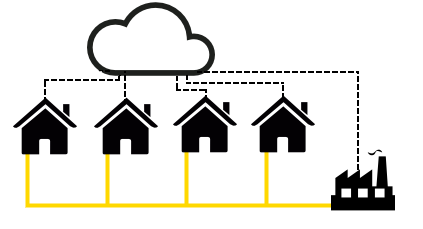
\includegraphics[width=0.6\textwidth]{billeder/CaseIlu.png}}

\put(177,110){Network}

\put(122,62){\color{white} \textbf{10}}
\put(174,62){\color{white} \textbf{13}}
\put(226,62){\color{white} \textbf{18}}
\put(276,62){\color{white} \textbf{23}}
\put(200,0){Power Line}

\end{picture}
\caption{The city setup}
\label{fig:CaseSetup}
\end{figure}

The city setup is illustrated in figure \ref{fig:CaseSetup}. The figure illustrates how the electric company supplies energy to the houses. All the houses have smart meters, and are informing the power company about the current consumption of each house, using some network. This is a fairly simplified example of a smart grid, that exists in many cities today. In this case it is assumed that the electric company receives information about the consumption of the houses each 30 seconds, as in the SmartHG dataset. Even though many smart meters today are capable of delivering information at this speed, it is more common to only get information each hour. This is mainly because the information is used to regulate distribution and production, which is a slow process that would not improve by faster update rates.  

The electric companies collect the information, and by using \ab{NILM} can calculate statistical information about the town. In the fictive case is a local TV station interested in knowing what time a day the citizens of the town watches TV, in a specific period, in order to improve some aspect of there product. 

\section{Methodology}
The aim of this case is to illustrate the potential of this kind of application for an electric company. Therefore is the data analysis conducted in a manner, that illustrates how an electric company could do it. This means that only the main meter information is used in the analysis, and the sub-meter information is only used to validate the results.  The goal is for the electric company to disaggregate the TV signals from the main meter signal, in order to use it in some statistical analysis. 

\begin{figure}[H]
\centering
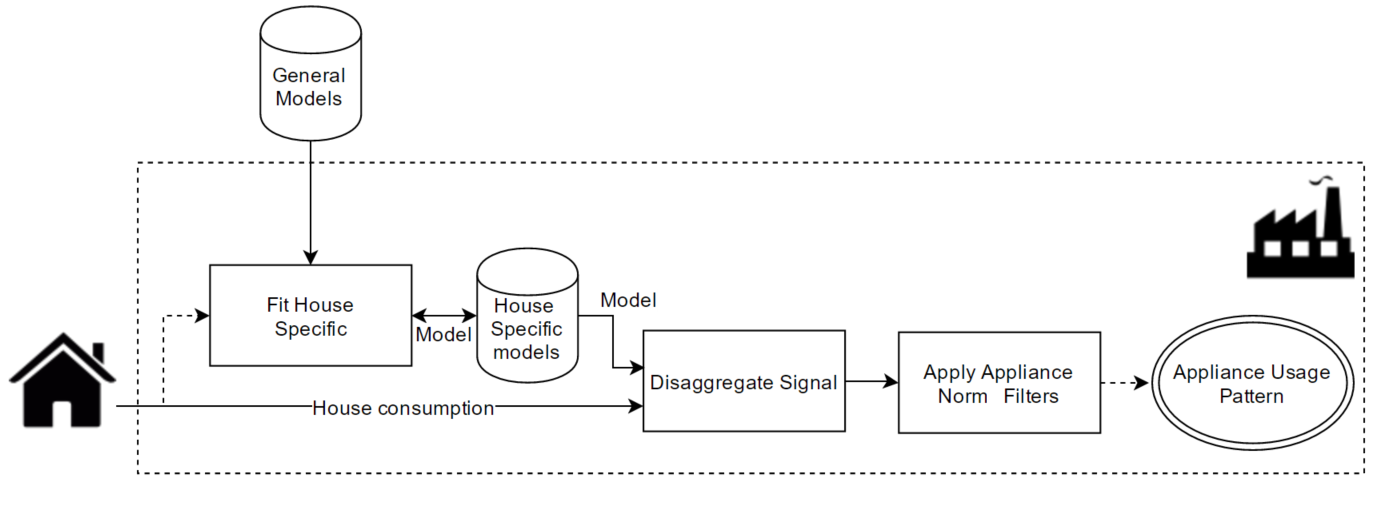
\includegraphics[width=1\textwidth]{billeder/Electric company method.png}
\caption{The disaggregation process}
\label{fig:ECM}
\end{figure}

This process is illustrated in figure \ref{fig:ECM}. It is assumed that the power company have access to a very general statistical model of the TV. This model can come from some outside database, or be one that the electric company developed themselves. The first step is to create a household specific model, that is a specialisation of the general model. This could be done with sub-meter data, but to make the experiment more realistic is the fitting of the model done using only the aggregated data from the main meter. This is done using the same method as developed for the Parson algorithm \citep{RefWorks:28}. This method finds periods where an appliance is turned ON and OFF without any other appliances changing states, is detected. This on/off single event fragments are then mapped to specific appliances using the general model. When enough on/off single event fragments have been collected can this information be used to fit a more specific model. This can happen in a contentiously manner, where the specific model is improved as more data is collected.  

Using the specific models disaggregation of the main meter signal can now be achieved. The statistical models selected in this case are the \ab{FHMM}. As discussed in section \ref{sec:NOISE}, the models alone gives a very error prone signal in the \ab{FHMM}. The signal is therefore feed through a norm filter. As discussed in \ref{sec:NormFilter} can the information about how a user normally would use the appliance be used to filter the disaggregated data to obtain better results. 

The result of this process is an appliance usage pattern, that can be used by the electric company to derive various statistical properties.  

The experiment is conducted with four weeks of data been used to fit TV specific models for each house. The analysis for the TV station is conducted over a period of six weeks, that is not overlapping with the initial four training weeks. 

\section{Results}
The viewing habits of the small town obtained by the disaggregation analysis is compared with the actual viewing habit obtained from the sub-meter data. In figure \ref{fig:WHW} is the results shown for the first week.   

\begin{figure}[H]
\centering
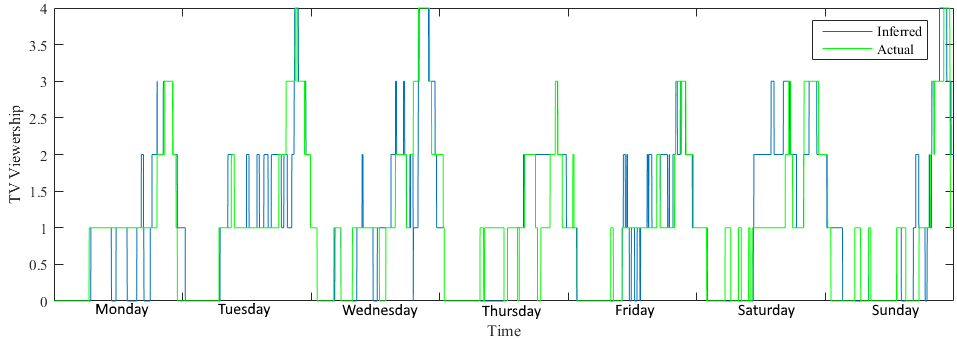
\includegraphics[width=1\textwidth]{billeder/Viewership.png}
\caption{Viewership in week one}
\label{fig:WHW}
\end{figure}

The figure shows the viewership, that tells how many in the city is watching TV at a given time. The green line is the actual viewership, where the blue is the viewership reported by the electric company. The results differer, as one would expect, since the disaggregation process in a noisy environment is a hard task. The general trends that many are watching TV in the evening, and not that many in the morning, is still represented nicely. This illustrates that the general trends of the viewership is maintained in the disaggregated signal, and this is commonly what is important for this kind of costumer statistics. 

In table \ref{tab:CaseRes} is the average number of viewers in 3 hour timeslots shown. The results shown in the table is the average of all 6 weeks, split up in the different weekdays. 

% Please add the following required packages to your document preamble:
% \usepackage{multirow}
\begin{table}[H]
\centering
\begin{tabular}{lccccccccc}
\cline{3-10}
                                                & \multicolumn{1}{c|}{}         & \multicolumn{8}{c|}{Time of day}                                                                                                                                                                                                                                                                              \\ \cline{3-10} 
                                                & \multicolumn{1}{c|}{}         & \multicolumn{1}{c|}{\textbf{00-03}} & \multicolumn{1}{c|}{\textbf{03-06}} & \multicolumn{1}{c|}{\textbf{06-09}} & \multicolumn{1}{c|}{\textbf{09-12}} & \multicolumn{1}{c|}{\textbf{12-13}} & \multicolumn{1}{c|}{\textbf{15-18}} & \multicolumn{1}{c|}{\textbf{18-21}} & \multicolumn{1}{c|}{\textbf{21-00}} \\ \cline{3-10} 
                                                &                               &                                     &                                     &                                     &                                     &                                     &                                     &                                     &                                     \\ \cline{2-10} 
\multicolumn{1}{l|}{\multirow{2}{*}{Monday}}    & \multicolumn{1}{c|}{Inferred} & \multicolumn{1}{c|}{0.12}           & \multicolumn{1}{c|}{0.00}           & \multicolumn{1}{c|}{0.66}           & \multicolumn{1}{c|}{1.19}           & \multicolumn{1}{c|}{1.02}           & \multicolumn{1}{c|}{1.31}           & \multicolumn{1}{c|}{2.39}           & \multicolumn{1}{c|}{2.08}           \\ \cline{2-10} 
\multicolumn{1}{l|}{}                           & \multicolumn{1}{c|}{True}     & \multicolumn{1}{c|}{0.13}           & \multicolumn{1}{c|}{0.28}           & \multicolumn{1}{c|}{0.98}           & \multicolumn{1}{c|}{0.87}           & \multicolumn{1}{c|}{0.68}           & \multicolumn{1}{c|}{1.28}           & \multicolumn{1}{c|}{2.49}           & \multicolumn{1}{c|}{1.72}           \\ \cline{2-10} 
                                                &                               &                                     &                                     &                                     &                                     &                                     &                                     &                                     &                                     \\ \cline{2-10} 
\multicolumn{1}{l|}{\multirow{2}{*}{Tuesday}}   & \multicolumn{1}{c|}{Inferred} & \multicolumn{1}{c|}{0.13}           & \multicolumn{1}{c|}{0.28}           & \multicolumn{1}{c|}{0.98}           & \multicolumn{1}{c|}{0.87}           & \multicolumn{1}{c|}{0.68}           & \multicolumn{1}{c|}{1.28}           & \multicolumn{1}{c|}{2.49}           & \multicolumn{1}{c|}{1.72}           \\ \cline{2-10} 
\multicolumn{1}{l|}{}                           & \multicolumn{1}{c|}{True}     & \multicolumn{1}{c|}{0.19}           & \multicolumn{1}{c|}{0.09}           & \multicolumn{1}{c|}{0.39}           & \multicolumn{1}{c|}{0.88}           & \multicolumn{1}{c|}{0.73}           & \multicolumn{1}{c|}{1.24}           & \multicolumn{1}{c|}{2.23}           & \multicolumn{1}{c|}{2.26}           \\ \cline{2-10} 
                                                &                               &                                     &                                     &                                     &                                     &                                     &                                     &                                     &                                     \\ \cline{2-10} 
\multicolumn{1}{l|}{\multirow{2}{*}{Wednesday}} & \multicolumn{1}{c|}{Inferred} & \multicolumn{1}{c|}{0.19}           & \multicolumn{1}{c|}{0.09}           & \multicolumn{1}{c|}{0.39}           & \multicolumn{1}{c|}{0.88}           & \multicolumn{1}{c|}{0.73}           & \multicolumn{1}{c|}{1.24}           & \multicolumn{1}{c|}{2.23}           & \multicolumn{1}{c|}{2.26}           \\ \cline{2-10} 
\multicolumn{1}{l|}{}                           & \multicolumn{1}{c|}{True}     & \multicolumn{1}{c|}{0.09}           & \multicolumn{1}{c|}{0.30}           & \multicolumn{1}{c|}{0.58}           & \multicolumn{1}{c|}{0.79}           & \multicolumn{1}{c|}{0.77}           & \multicolumn{1}{c|}{1.42}           & \multicolumn{1}{c|}{2.72}           & \multicolumn{1}{c|}{2.11}           \\ \cline{2-10} 
\multicolumn{1}{c}{}                            &                               &                                     &                                     &                                     &                                     &                                     &                                     &                                     &                                     \\ \cline{2-10} 
\multicolumn{1}{l|}{\multirow{2}{*}{Thursday}}  & \multicolumn{1}{c|}{Inferred} & \multicolumn{1}{c|}{0.09}           & \multicolumn{1}{c|}{0.30}           & \multicolumn{1}{c|}{0.58}           & \multicolumn{1}{c|}{0.79}           & \multicolumn{1}{c|}{0.77}           & \multicolumn{1}{c|}{1.42}           & \multicolumn{1}{c|}{2.72}           & \multicolumn{1}{c|}{2.11}           \\ \cline{2-10} 
\multicolumn{1}{l|}{}                           & \multicolumn{1}{c|}{True}     & \multicolumn{1}{c|}{0.12}           & \multicolumn{1}{c|}{0.09}           & \multicolumn{1}{c|}{0.31}           & \multicolumn{1}{c|}{0.96}           & \multicolumn{1}{c|}{1.12}           & \multicolumn{1}{c|}{1.69}           & \multicolumn{1}{c|}{2.86}           & \multicolumn{1}{c|}{2.30}           \\ \cline{2-10} 
                                                &                               &                                     &                                     &                                     &                                     &                                     &                                     &                                     &                                     \\ \cline{2-10} 
\multicolumn{1}{l|}{\multirow{2}{*}{Friday}}    & \multicolumn{1}{c|}{Inferred} & \multicolumn{1}{c|}{0.12}           & \multicolumn{1}{c|}{0.09}           & \multicolumn{1}{c|}{0.31}           & \multicolumn{1}{c|}{0.96}           & \multicolumn{1}{c|}{1.12}           & \multicolumn{1}{c|}{1.69}           & \multicolumn{1}{c|}{2.86}           & \multicolumn{1}{c|}{2.30}           \\ \cline{2-10} 
\multicolumn{1}{l|}{}                           & \multicolumn{1}{c|}{True}     & \multicolumn{1}{c|}{0.10}           & \multicolumn{1}{c|}{0.18}           & \multicolumn{1}{c|}{0.66}           & \multicolumn{1}{c|}{0.91}           & \multicolumn{1}{c|}{0.74}           & \multicolumn{1}{c|}{1.65}           & \multicolumn{1}{c|}{3.17}           & \multicolumn{1}{c|}{2.35}           \\ \cline{2-10} 
                                                &                               &                                     &                                     &                                     &                                     &                                     &                                     &                                     &                                     \\ \cline{2-10} 
\multicolumn{1}{l|}{\multirow{2}{*}{Saturday}}  & \multicolumn{1}{c|}{Inferred} & \multicolumn{1}{c|}{0.10}           & \multicolumn{1}{c|}{0.18}           & \multicolumn{1}{c|}{0.66}           & \multicolumn{1}{c|}{0.91}           & \multicolumn{1}{c|}{0.74}           & \multicolumn{1}{c|}{1.65}           & \multicolumn{1}{c|}{3.17}           & \multicolumn{1}{c|}{2.35}           \\ \cline{2-10} 
\multicolumn{1}{l|}{}                           & \multicolumn{1}{c|}{True}     & \multicolumn{1}{c|}{0.28}           & \multicolumn{1}{c|}{0.17}           & \multicolumn{1}{c|}{0.95}           & \multicolumn{1}{c|}{0.77}           & \multicolumn{1}{c|}{1.39}           & \multicolumn{1}{c|}{1.36}           & \multicolumn{1}{c|}{2.26}           & \multicolumn{1}{c|}{2.10}           \\ \cline{2-10} 
                                                &                               &                                     &                                     &                                     &                                     &                                     &                                     &                                     &                                     \\ \cline{2-10} 
\multicolumn{1}{l|}{\multirow{2}{*}{Sunday}}    & \multicolumn{1}{c|}{Inferred} & \multicolumn{1}{c|}{0.28}           & \multicolumn{1}{c|}{0.17}           & \multicolumn{1}{c|}{0.95}           & \multicolumn{1}{c|}{0.77}           & \multicolumn{1}{c|}{1.39}           & \multicolumn{1}{c|}{1.36}           & \multicolumn{1}{c|}{2.26}           & \multicolumn{1}{c|}{2.10}           \\ \cline{2-10} 
\multicolumn{1}{l|}{}                           & \multicolumn{1}{c|}{True}     & \multicolumn{1}{c|}{0.12}           & \multicolumn{1}{c|}{0.00}           & \multicolumn{1}{c|}{1.01}           & \multicolumn{1}{c|}{0.96}           & \multicolumn{1}{c|}{0.96}           & \multicolumn{1}{c|}{1.33}           & \multicolumn{1}{c|}{1.93}           & \multicolumn{1}{c|}{1.65}           \\ \cline{2-10} 
\end{tabular}
\caption{Average viewership in a 6 week period.}
\label{tab:CaseRes}
\end{table}

This illustrates that the true trends in the information is maintained. The results indicates that it is in some degree possible to obtain user information from the disaggregated data. The TV is a relative hard appliance to detect, since there are many different types. The success in this experiment is partly due to the fact that the TV was some of the main consumers of the houses selected, and they had a pure Type-I behaviour.

\section{Chapter Discussion}
In this chapter was a very simple example of how the electric company can extend their product range to statistical information. This information could potentially also be used to extend their product range to their current costumers. One example of this could be a fridge surveillance system that would send warning messages to the resident if their fridge stopped working.

At the current state of \ab{NILM} is the information only limited to a small amount of devices, since it is hard other appliances than the top consumers in the household. One of the techniques shown to greatly improve the effectiveness of \ab{NILM} is to switch from the sub 1 Hz sampling range to a higher sampling rate in the kHz range. In the future where either meters capable of delivering information at high frequency is common in the houses or the \ab{NILM} techniques have advanced, it is a possibility for the electric companies to deliver very detailed user behavioural statistics. This information can be of interest for companies developing and selling electronics, since they are able to get accurate user reports about their products. 

